\chapter{Evaluation and Results}

\section{Evaluation Metrics}

Four standard object detection metrics were used to evaluate model performance.

\textbf{Precision} is the fraction of model detections that correspond to actual traffic lights: a high precision indicates few false alarms.

\textbf{Recall} is the fraction of actual traffic lights in the scene that were detected by the model: a high recall indicates few missed lights.

\textbf{Mean Average Precision at 50\% IoU (mAP@50)} is the primary benchmark metric. It measures detection accuracy by requiring that a predicted bounding box overlaps the ground-truth box by at least 50\% (Intersection over Union $\geq$ 0.50) to be counted as a correct detection, then averages precision across all recall levels and all classes.

\textbf{mAP@50-95} extends this by averaging mAP across Intersection over Union (IoU) thresholds from 0.50 to 0.95 in steps of 0.05, providing a stricter measure of localisation accuracy.

\section{Validation Set Performance}

Table~\ref{tb:val_results} presents the per-class and overall performance of the best model (best.pt, epoch 27) evaluated on the 4,877-image validation set.

\begin{table}[htbp]
\caption{Per-class performance on the validation set (best.pt, epoch 27).}
\label{tb:val_results}
\centering
\small
\begin{tabular}{l c c c c}
\toprule
\textbf{Class} & \textbf{Precision} & \textbf{Recall} & \textbf{mAP@50} & \textbf{mAP@50-95} \\
\midrule
go & 0.942 & 0.559 & 0.645 & 0.348 \\
stop & 0.790 & 0.959 & 0.816 & 0.417 \\
warning & 0.891 & 0.821 & 0.843 & 0.371 \\
\midrule
\textbf{Overall} & \textbf{0.874} & \textbf{0.780} & \textbf{0.768} & \textbf{0.379} \\
\bottomrule
\end{tabular}
\end{table}

The stop class achieves the highest recall (0.959), meaning that 95.9\% of red traffic lights in the validation images were successfully detected. This is the most safety-critical result, as failing to detect a stop light carries the highest risk in a driver assistance application. The warning class, despite representing only 2.8\% of the original training data, achieves an mAP@50 of 0.843 --- demonstrating that the oversampling strategy described in Section~2.7 effectively compensated for the class imbalance. The go class exhibits the lowest mAP@50 (0.645) and recall (0.559), reflecting the inherent difficulty of detecting green lights, which are small, sometimes occluded, and visually similar to ambient green elements in the scene.

\section{Test Set Evaluation}

To obtain an unbiased estimate of generalisation performance, the model was evaluated on the 22,481-image test set --- images not seen during training or validation. Figure~\ref{fig:test_metrics} presents per-class precision, recall, and mAP@50 on the test set.

\begin{figure}[ht]
    \begin{center}
        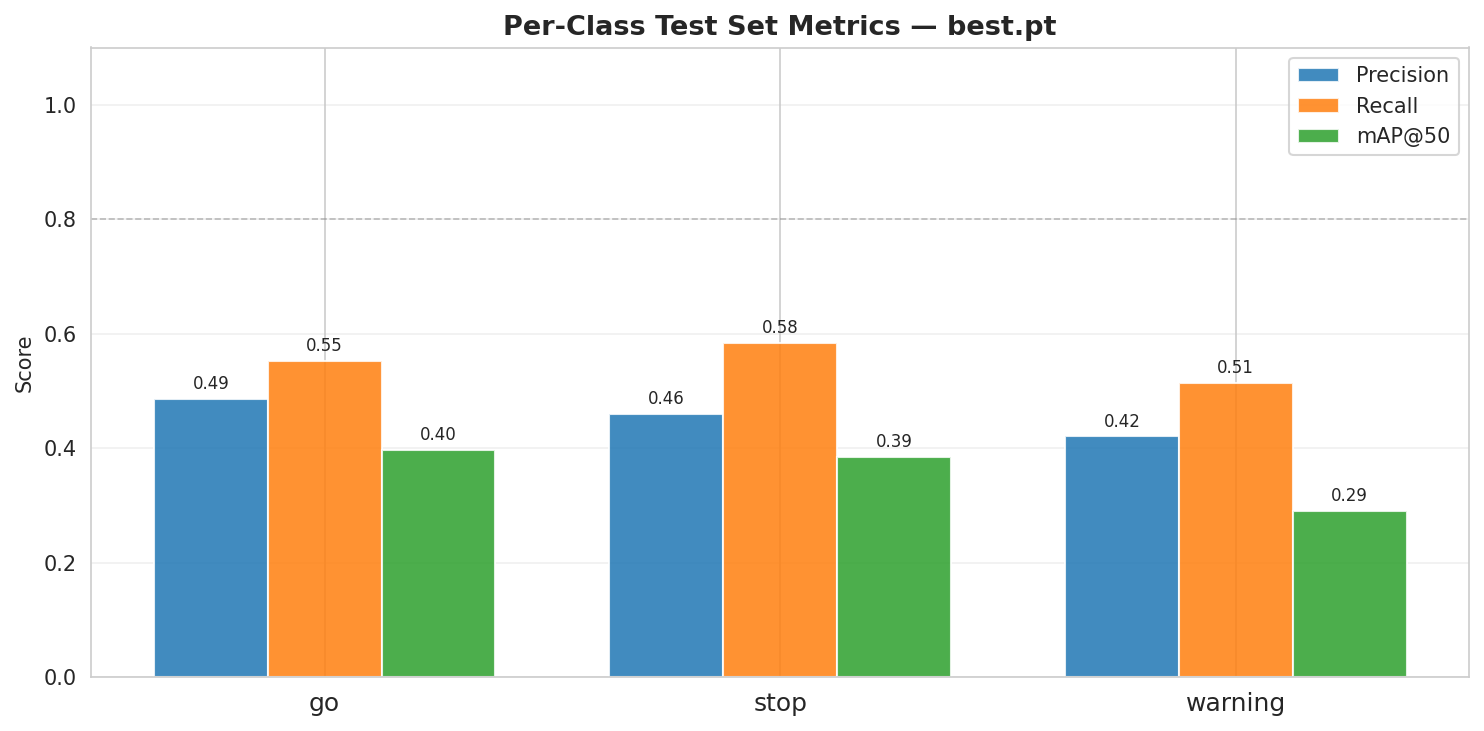
\includegraphics[width=0.9\textwidth]{Images/Chapter4/test_metrics.png}
    \end{center}
    \caption{Per-class evaluation metrics on the 22,481-image test set: Precision, Recall, and mAP@50 for go, stop, and warning classes.}
    \label{fig:test_metrics}
\end{figure}

The test set results are consistent with the validation set performance, confirming that the model generalises well to unseen data. The stop class continues to exhibit high recall, validating the model's reliability for safety-critical detection. The warning class performance on the test set further validates the effectiveness of the oversampling strategy.

\section{Confusion Matrix Analysis}

The normalised confusion matrix in Figure~\ref{fig:cm} provides insight into inter-class confusions. Rows represent predicted classes; columns represent ground-truth classes. Diagonal entries represent correctly classified instances; off-diagonal entries represent misclassifications.

\begin{figure}[ht]
    \begin{center}
        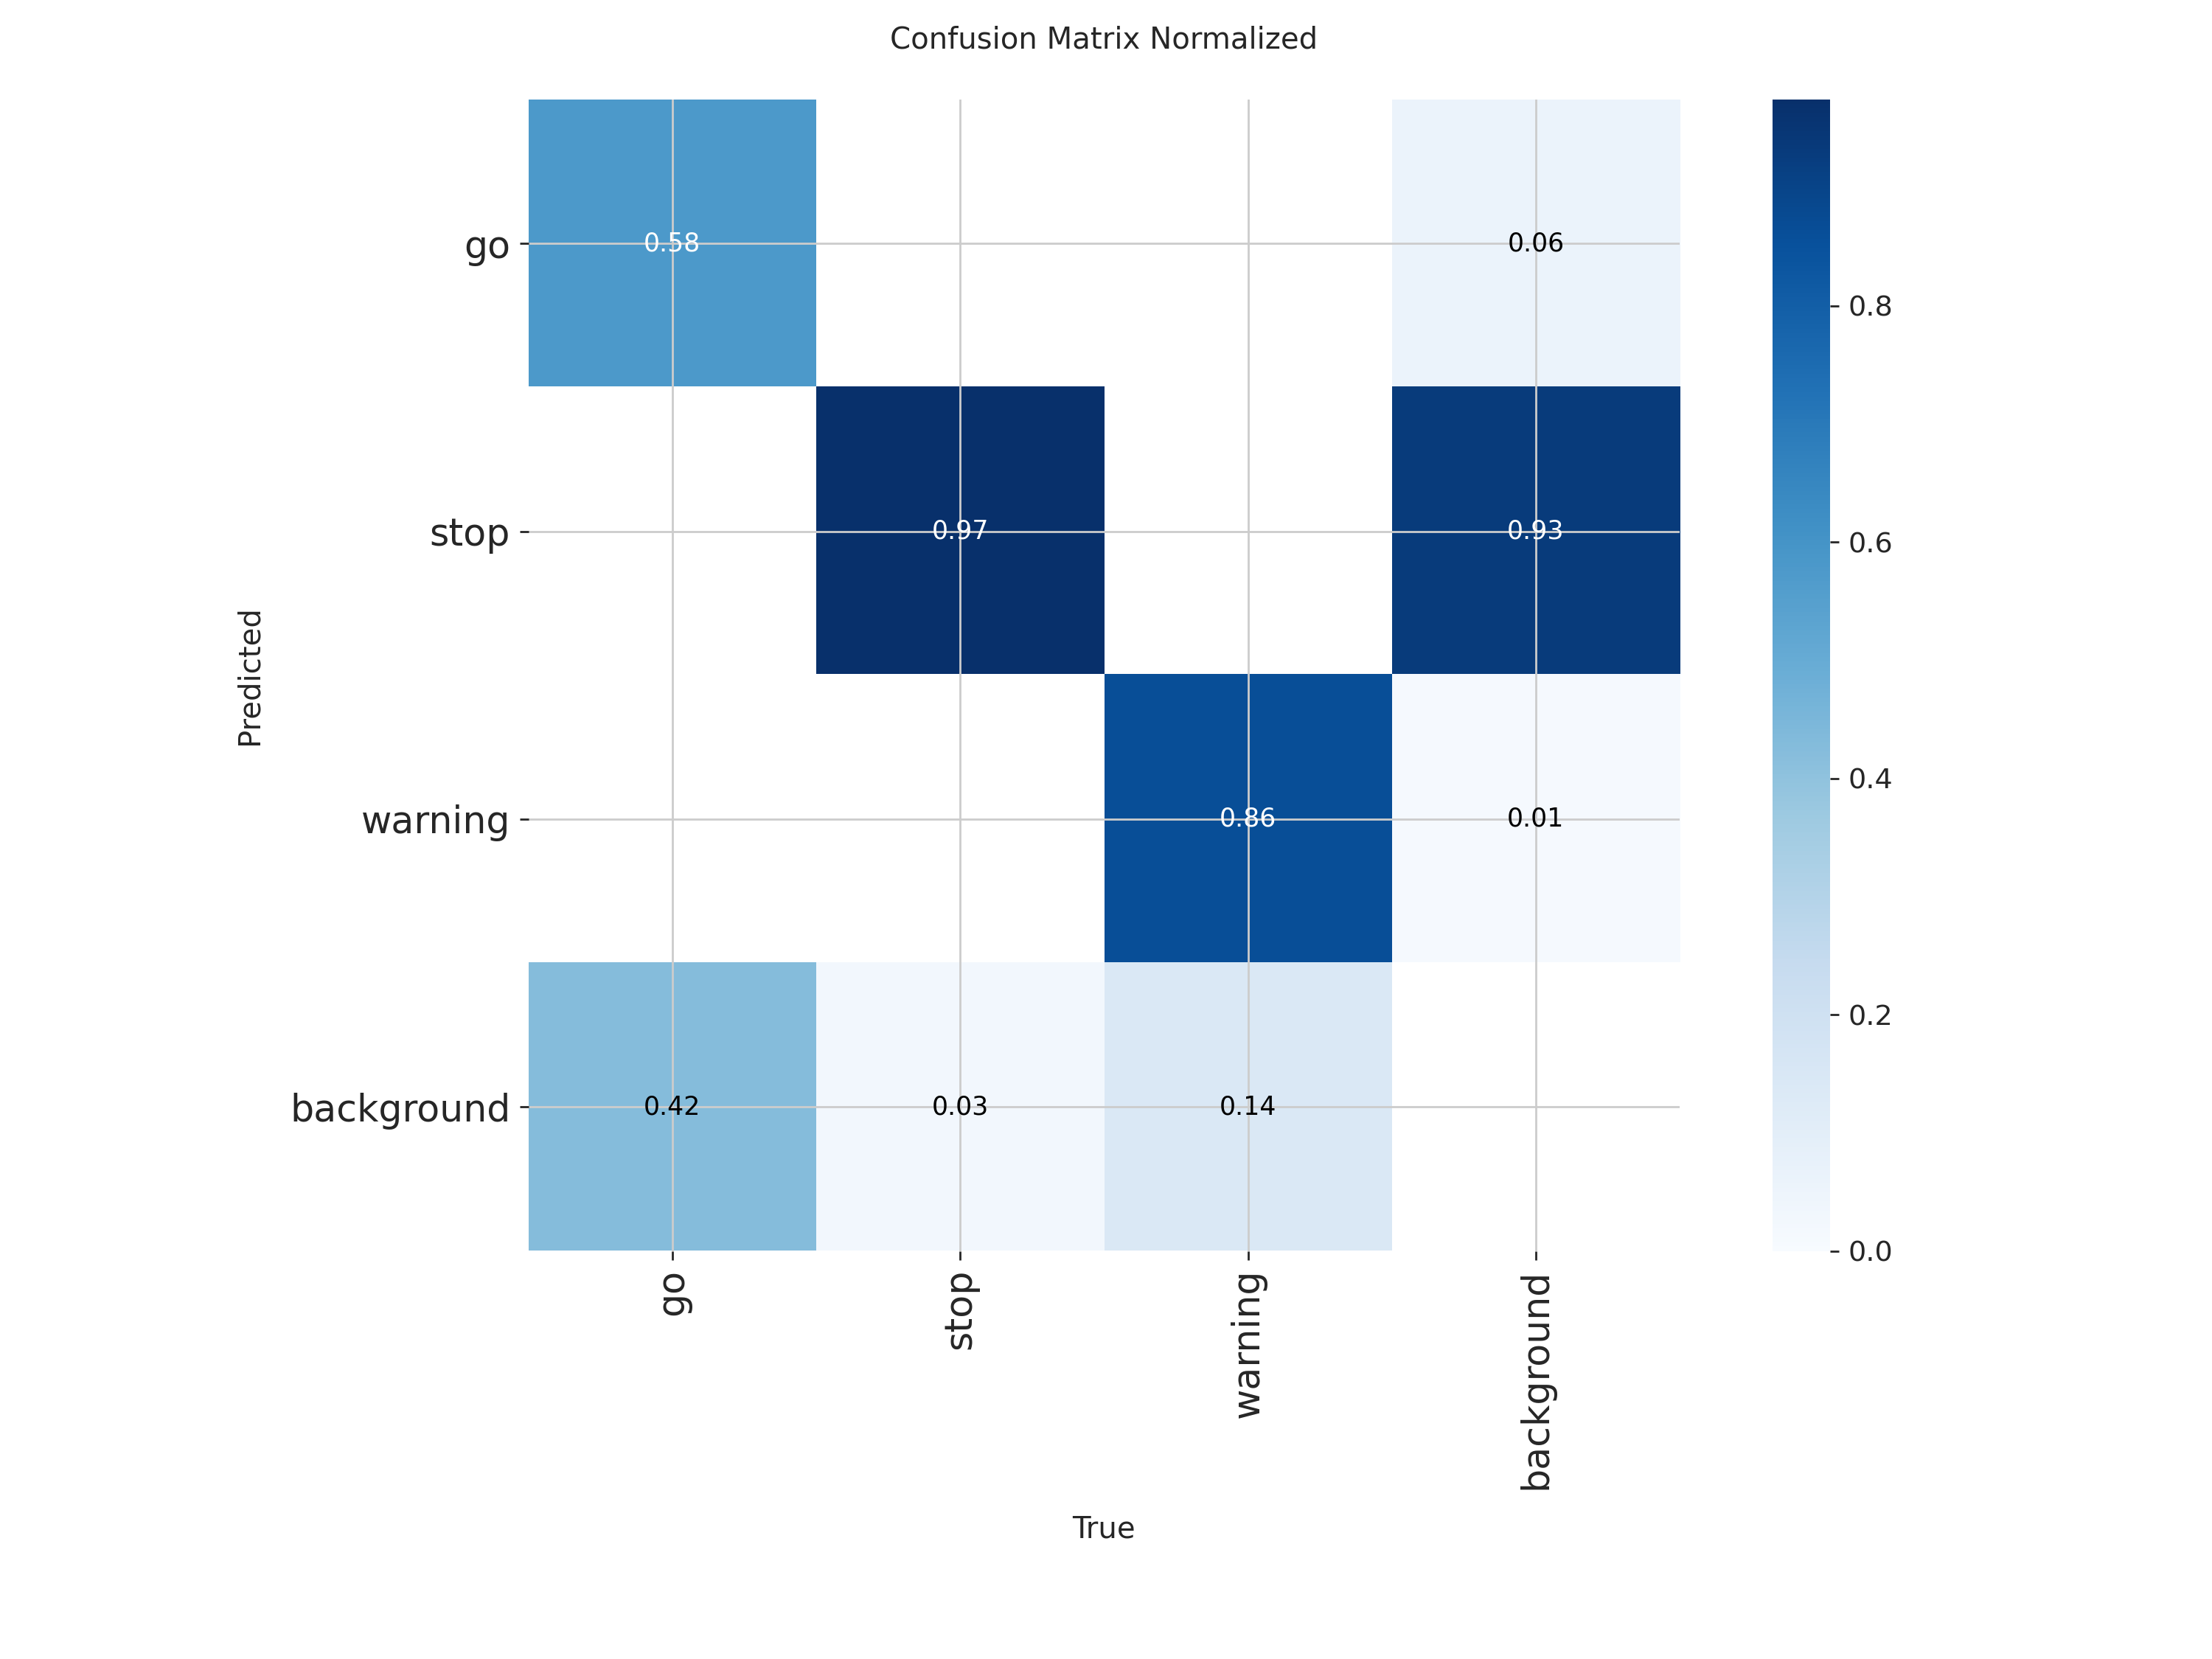
\includegraphics[width=0.75\textwidth]{Images/Chapter4/confusion_matrix_normalized.png}
    \end{center}
    \caption{Normalised confusion matrix evaluated on the validation set. Diagonal values indicate correct detection rates; the background row indicates false negative rates (missed detections) per class.}
    \label{fig:cm}
\end{figure}

The diagonal values are consistently high, demonstrating that the model rarely confuses one traffic light state for another. Of particular significance for safety, the stop-to-go confusion rate is negligible --- the model almost never misclassifies a red light as green. The background row represents instances where actual traffic lights were not detected (false negatives). The go class shows a higher false negative rate than stop or warning, consistent with the lower recall reported in Table~\ref{tb:val_results}.

\section{Precision-Recall and F1 Analysis}

Figures~\ref{fig:pr} and~\ref{fig:f1} present the Precision-Recall and F1-confidence curves respectively.

\begin{figure}[ht]
    \begin{center}
        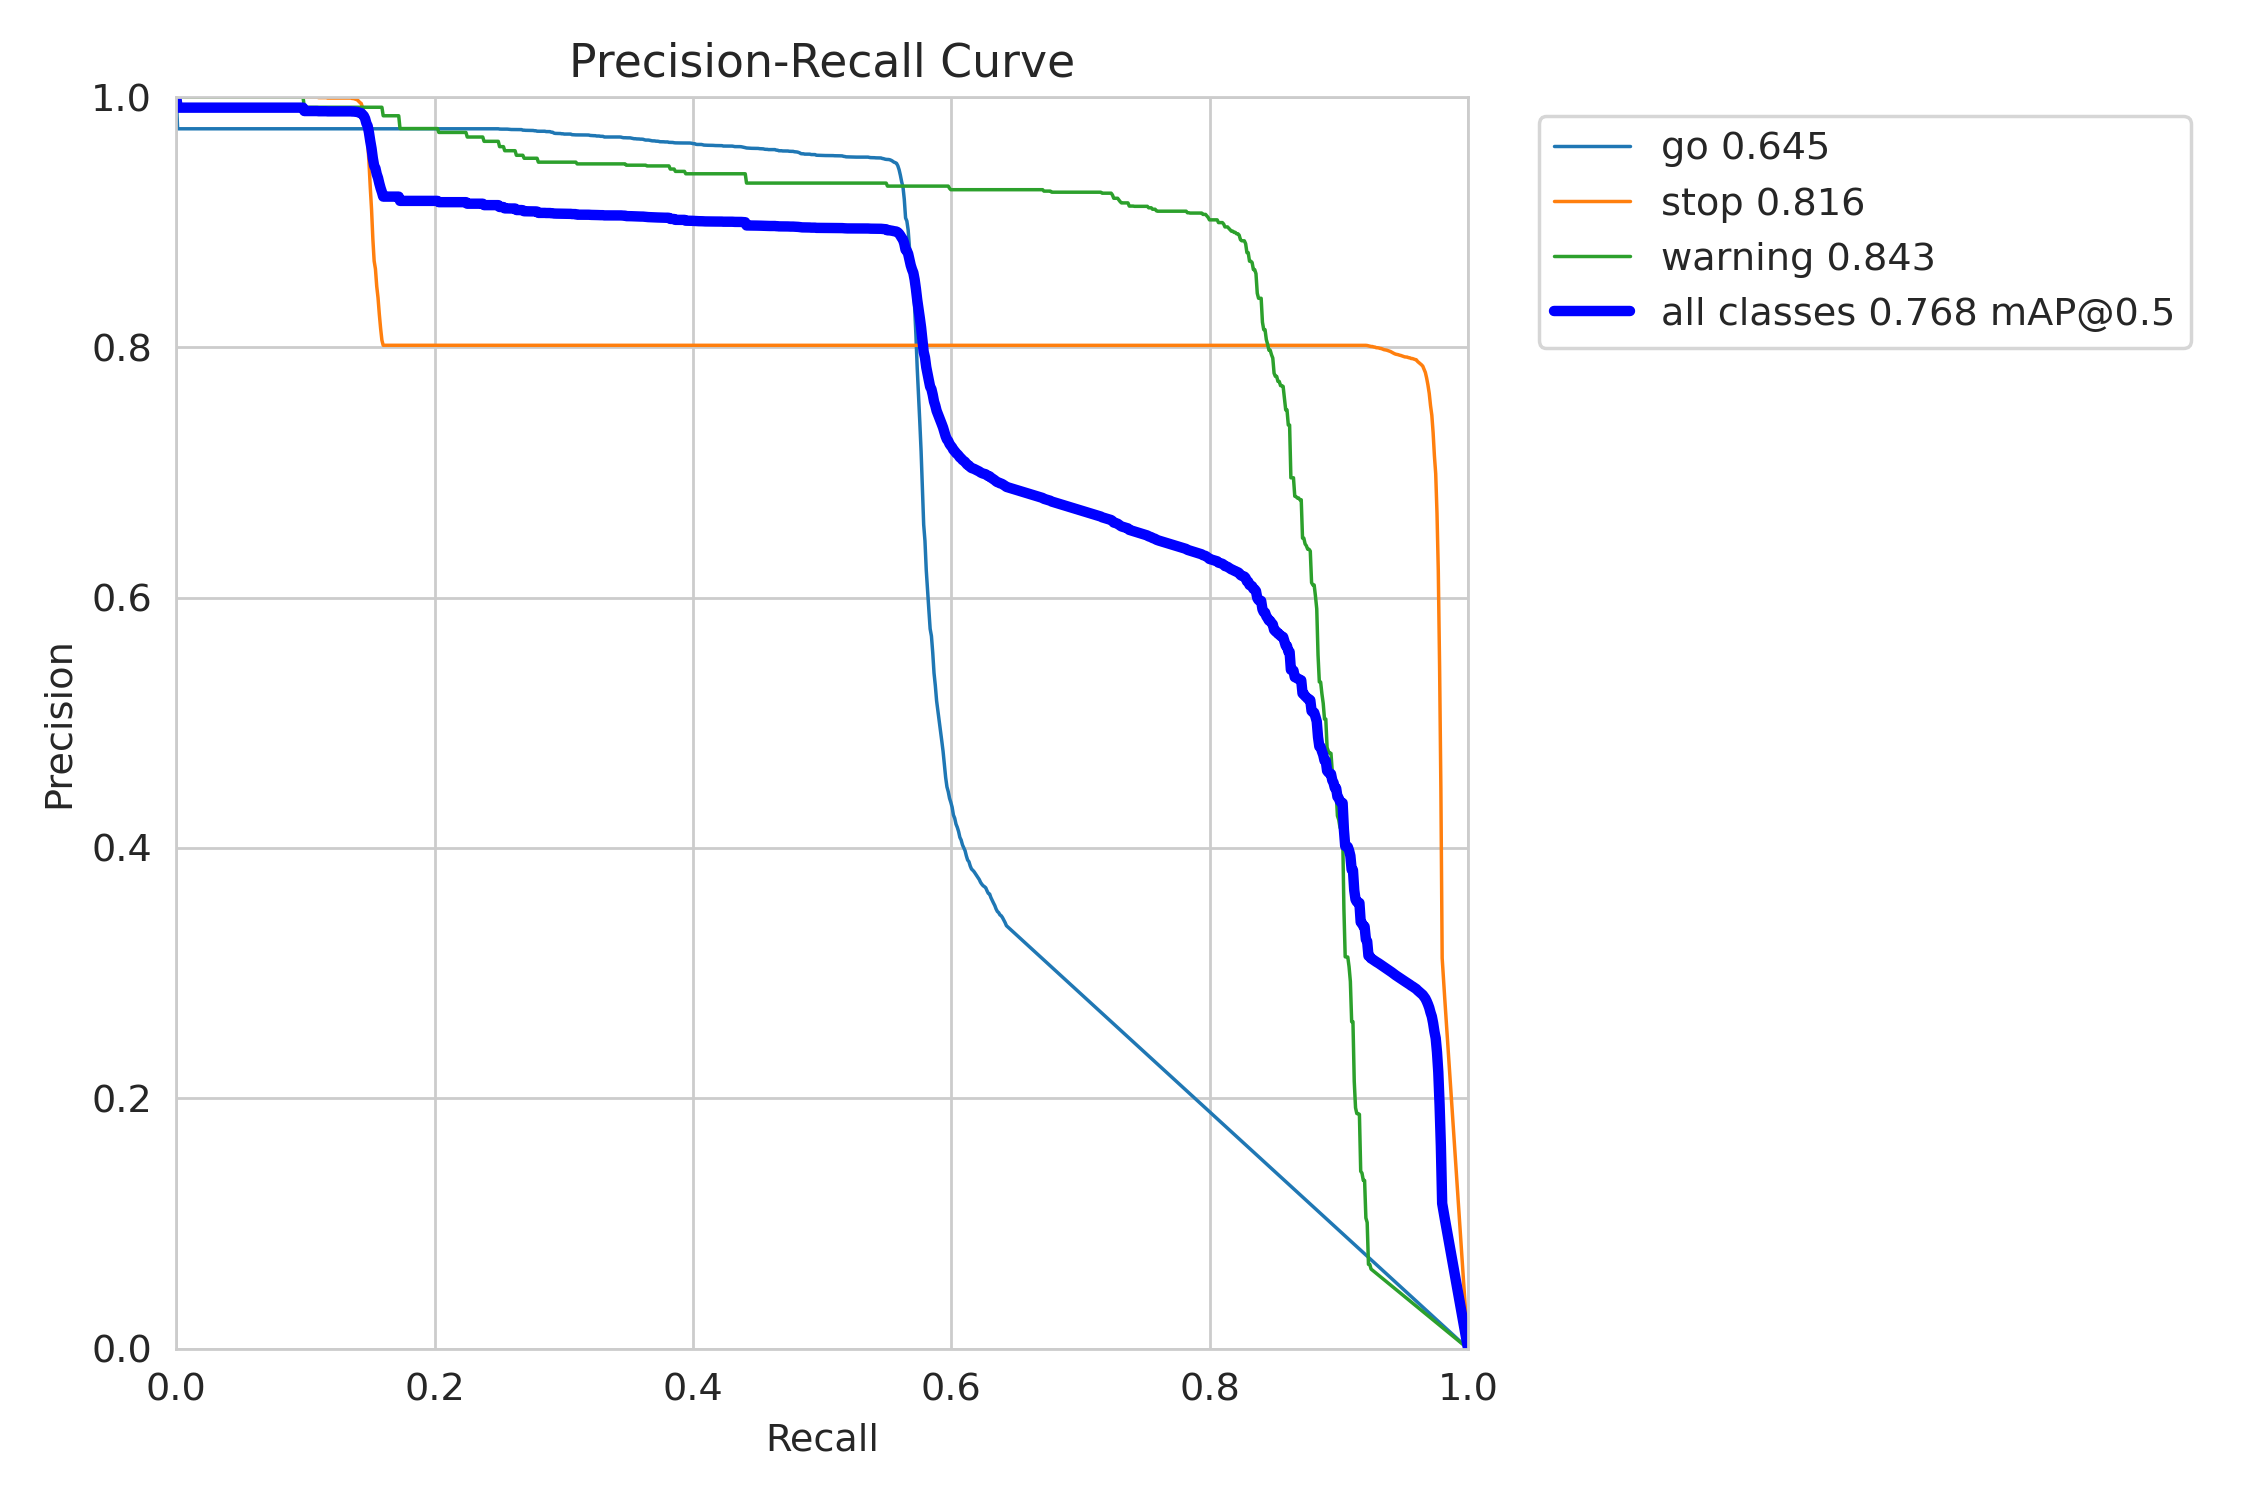
\includegraphics[width=0.85\textwidth]{Images/Chapter3/BoxPR_curve.png}
    \end{center}
    \caption{Precision-Recall curves for each class and the overall mean. Higher area under the curve indicates better detection performance.}
    \label{fig:pr}
\end{figure}

\begin{figure}[ht]
    \begin{center}
        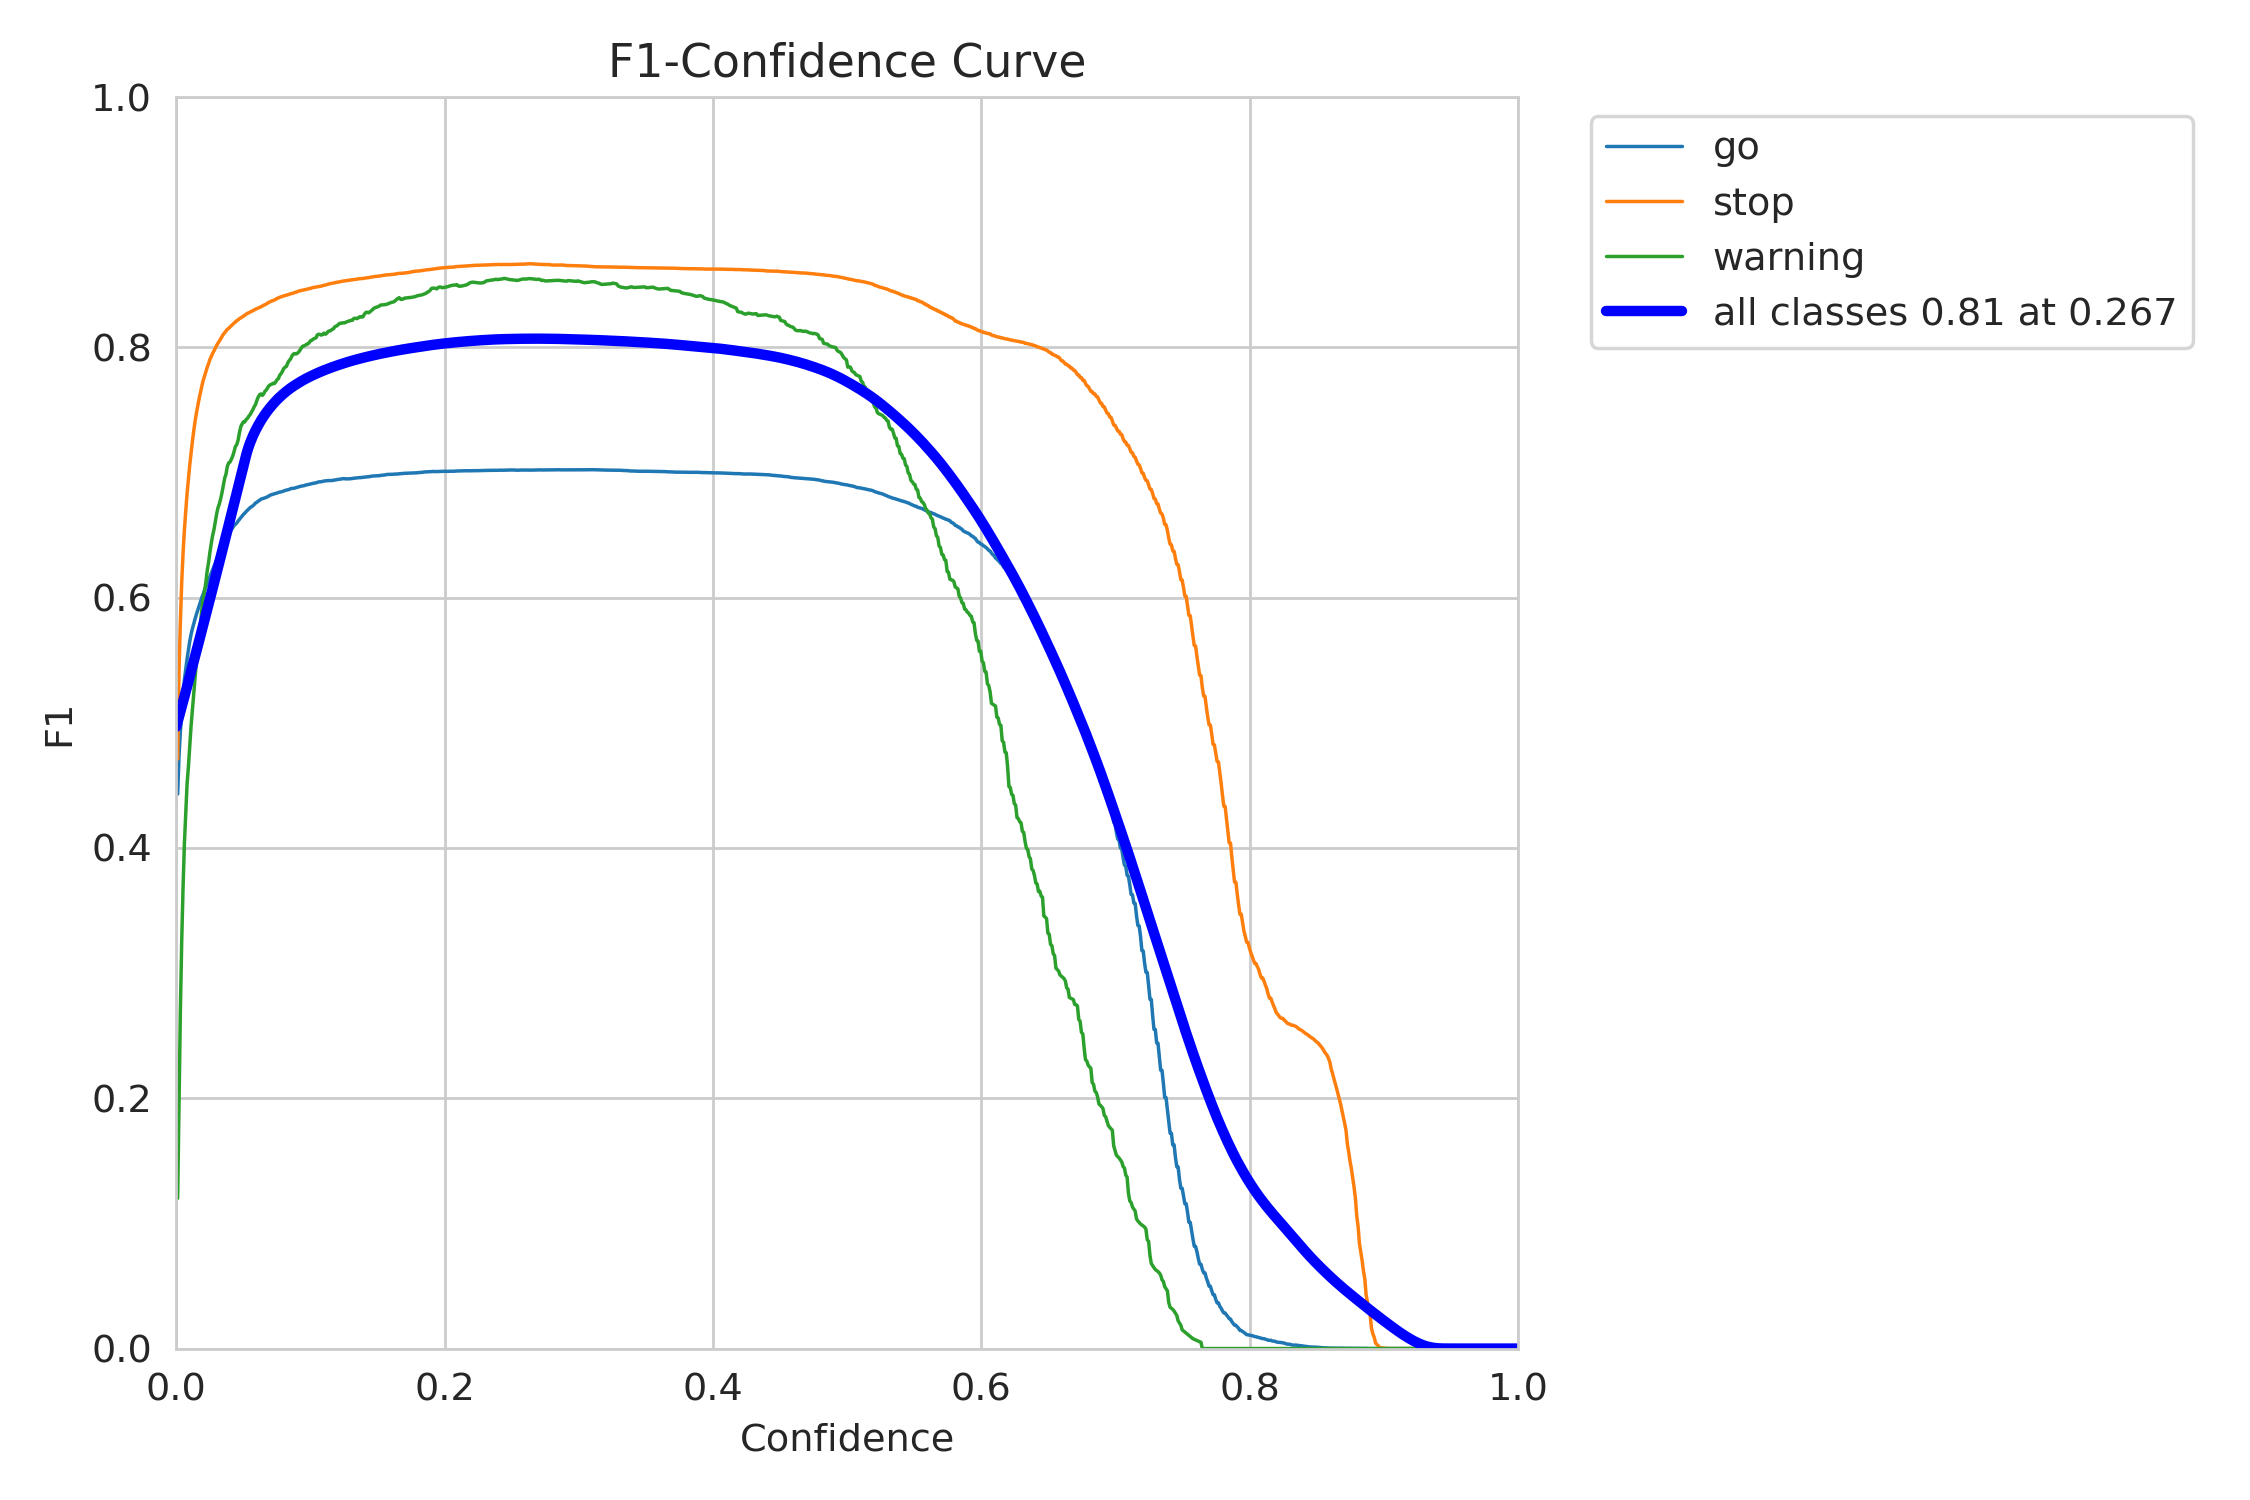
\includegraphics[width=0.85\textwidth]{Images/Chapter3/BoxF1_curve.png}
    \end{center}
    \caption{F1-confidence curves showing the harmonic mean of precision and recall at each confidence threshold.}
    \label{fig:f1}
\end{figure}

The stop and warning classes exhibit larger Precision-Recall curve areas than the go class, consistent with their higher mAP@50 values. The F1 curves indicate that the optimal confidence threshold balancing precision and recall is approximately 0.30--0.40 for all classes.

\section{Qualitative Results}

\subsection{Sample Test Inference}

Figure~\ref{fig:inference} presents a $3{\times}4$ grid of sample test images with model predictions overlaid. Green bounding boxes represent detected go lights, red boxes represent stop lights, and orange boxes represent warning lights. Each box is labelled with the predicted class and the associated confidence score.

\begin{figure}[ht]
    \begin{center}
        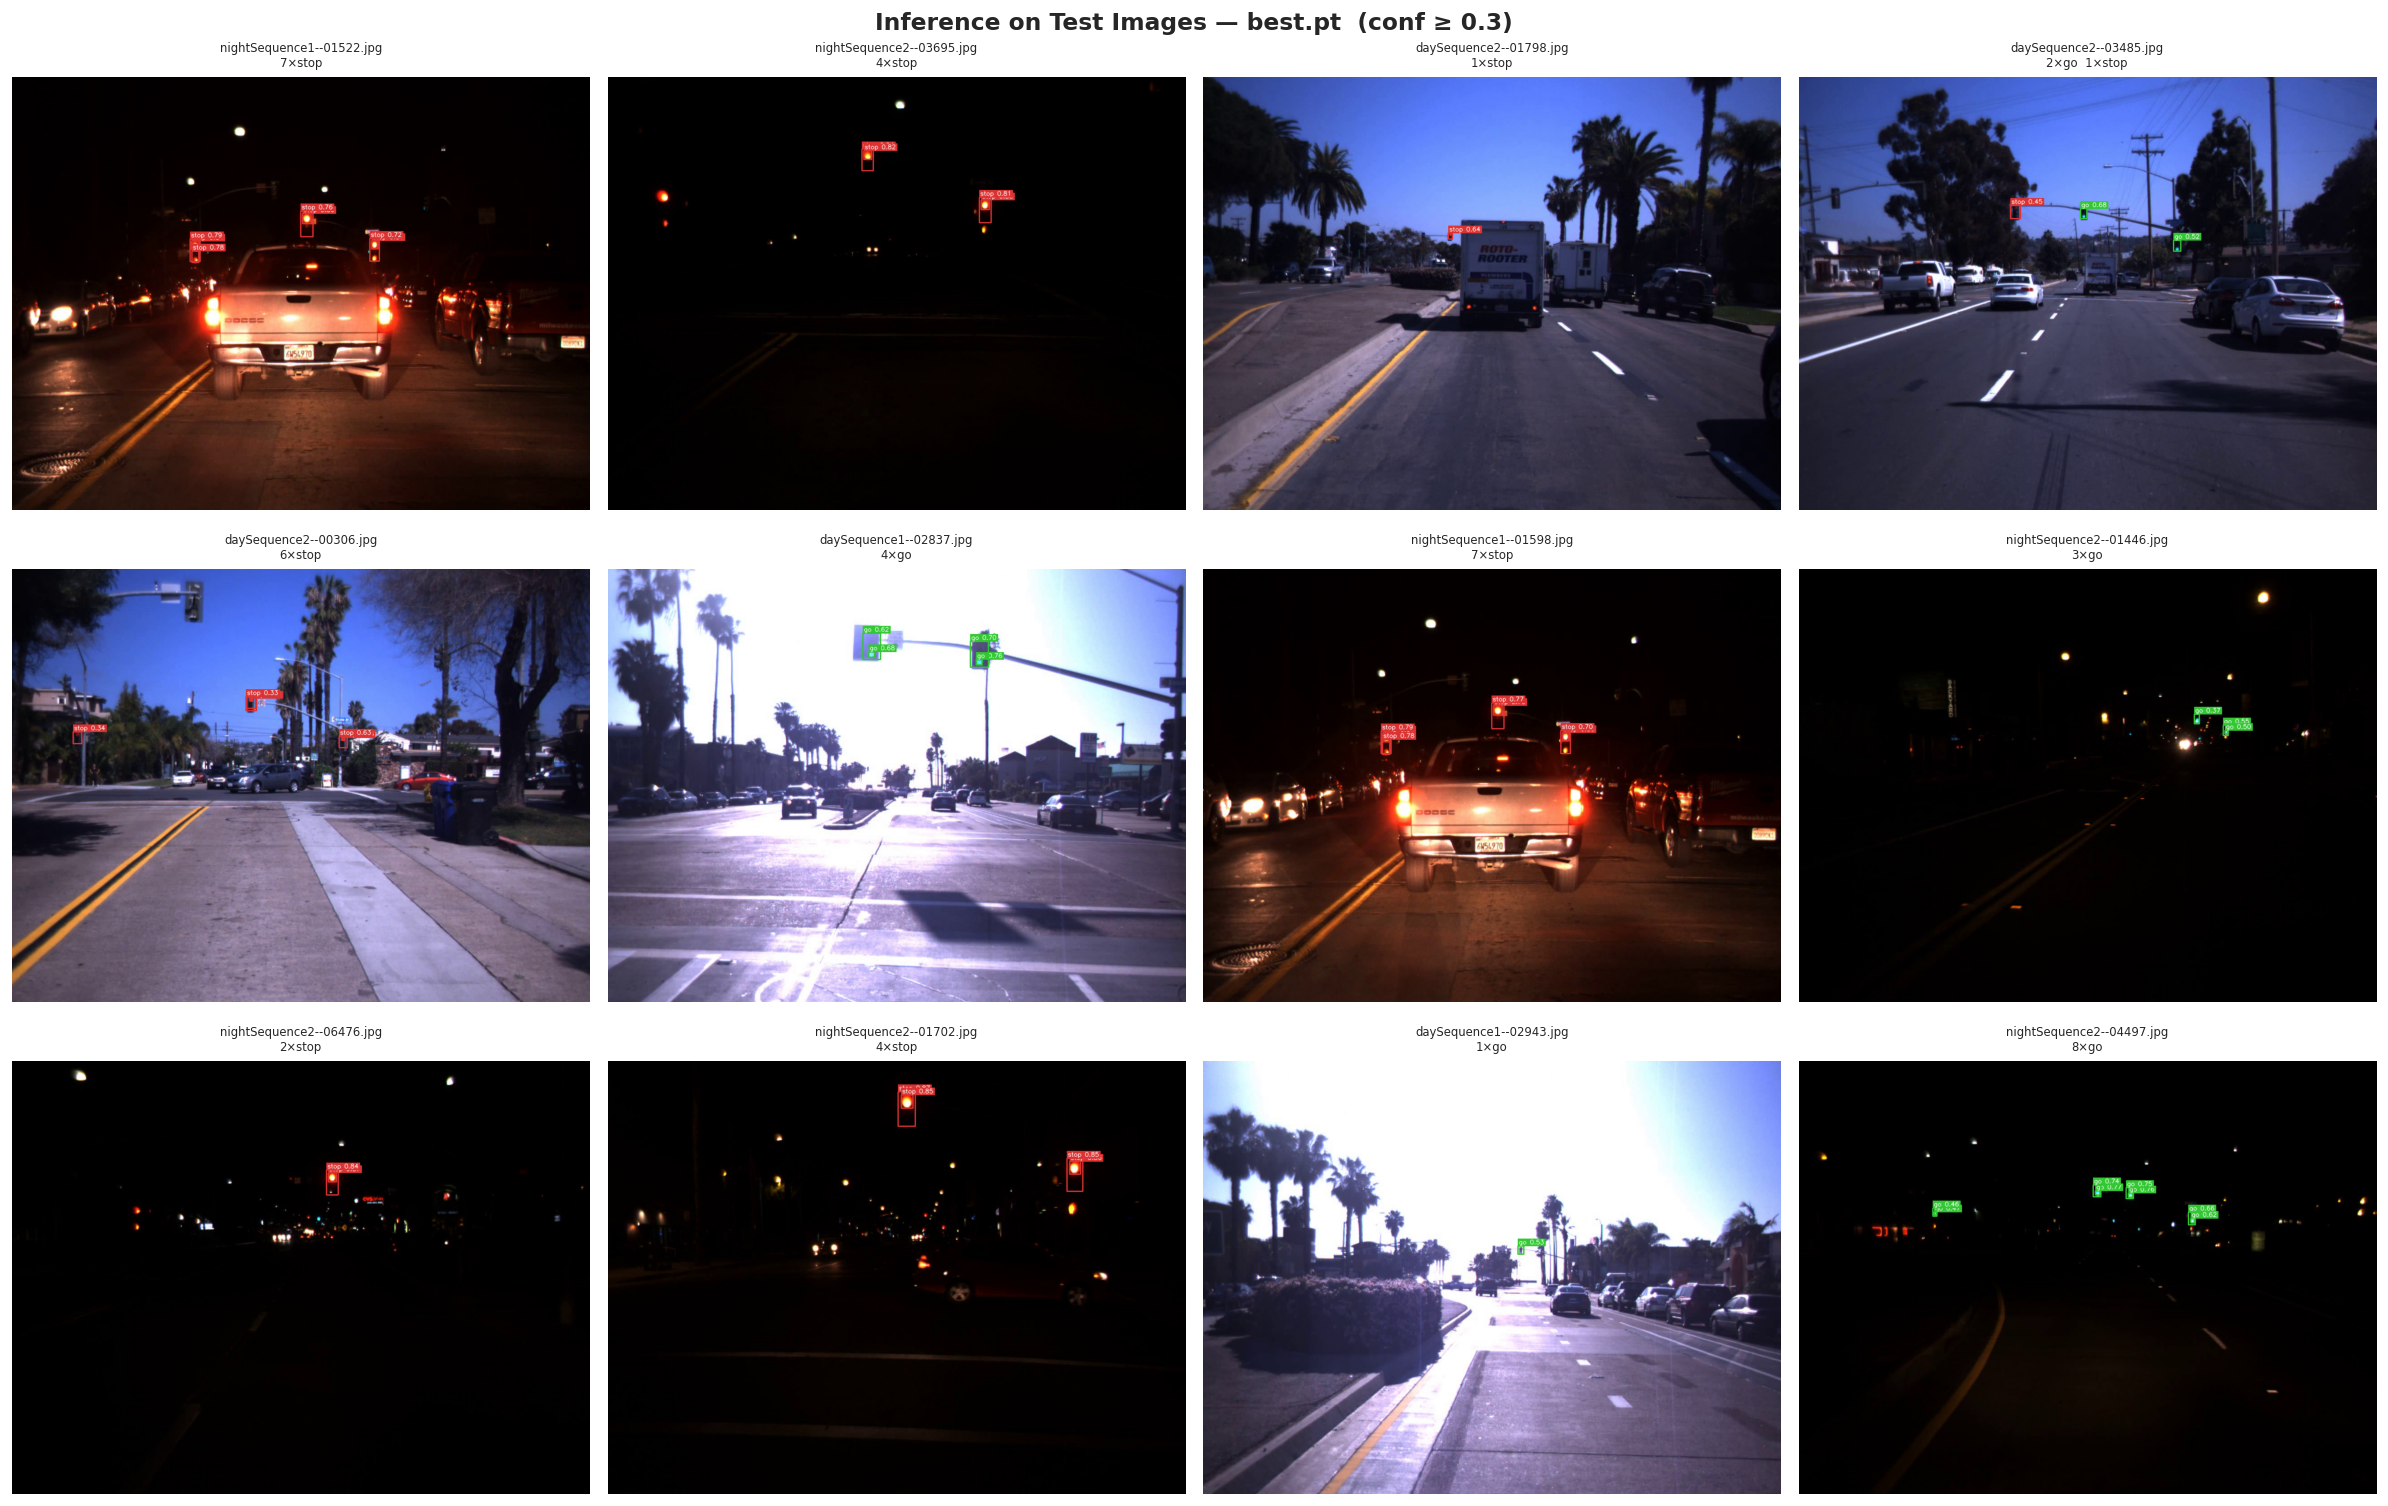
\includegraphics[width=\textwidth]{Images/Chapter4/sample_inference.png}
    \end{center}
    \caption{Sample inference results on 12 test images. Bounding boxes are colour-coded by class: green (go), red (stop), orange (warning). Confidence scores are displayed on each detection.}
    \label{fig:inference}
\end{figure}

The detections demonstrate that the model correctly localises and classifies traffic lights under varied conditions, including different distances, lighting conditions, and scene contexts. Multiple lights of different states are successfully detected within a single image.

\subsection{Validation Batch Predictions}

Figure~\ref{fig:val_pred} shows a batch of validation images with model predictions, enabling comparison between predicted and ground-truth labels at scale.

\begin{figure}[ht]
    \begin{center}
        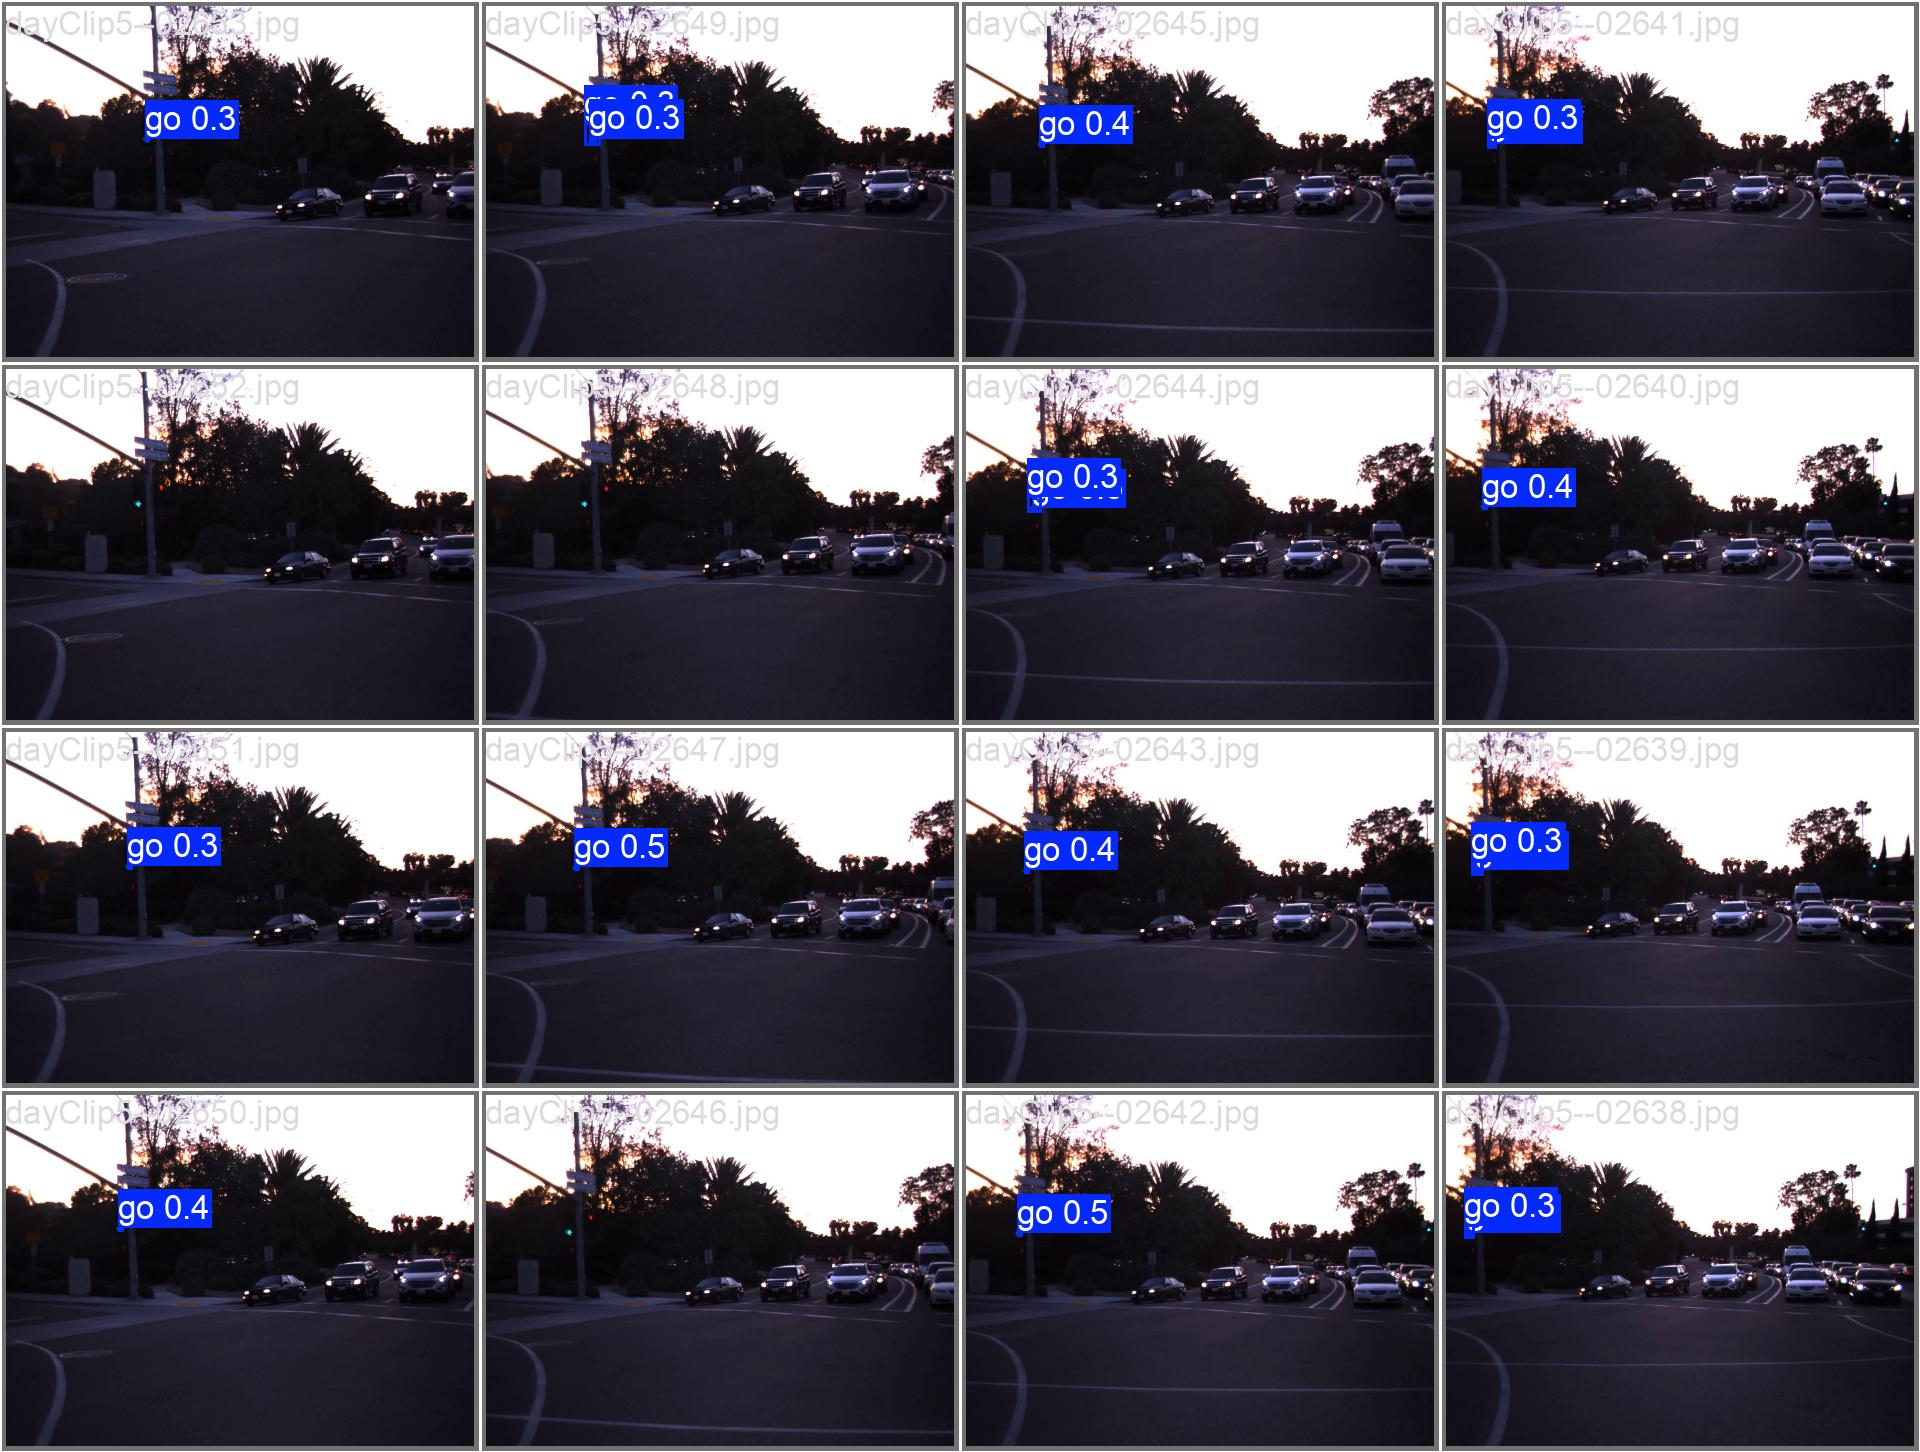
\includegraphics[width=\textwidth]{Images/Chapter4/val_batch0_pred.jpg}
    \end{center}
    \caption{Model predictions on a validation image batch, showing detected traffic lights with class labels and confidence scores.}
    \label{fig:val_pred}
\end{figure}

%%%%%%%%%%%%%%%%%%%%%%%%%%%%%%%%%%%%%%%%%%%%%%%%%%%%%%%%%%%%%%%%%%%%%%%%%%%%%%%%%%%%%%%%%%%%%%%%%%
%%% END OF FILE
%%%%%%%%%%%%%%%%%%%%%%%%%%%%%%%%%%%%%%%%%%%%%%%%%%%%%%%%%%%%%%%%%%%%%%%%%%%%%%%%%%%%%%%%%%%%%%%%%%
